\chapter{Introduction} \label{chap:intro}
``The most profound technologies are those that disappear'', Mark Weiser, Chief Technologist at Xerox PARC, famously wrote in his \textit{The Computer for the 21st Century} (\citeyear{weiser1991computer}) \cite{weiser1991computer}. Indeed, the vision of ubiquitous computing, or \mbox{\textbf{ubicomp}}, which he largely coined, is one where computers are invisible servants merged with the environment. They inform the user without requiring their attention, and controlling them is intuitive to the point where they feel like an extension of the user's unconsciousness rather than a tool \cite{weiser1997coming}.

One of the first examples of ubicomp was the now-famous \textit{Live Wire} or \textit{Dangling String}, shown in Figure \ref{fig:live_wire}. It is an ordinary piece or rope attached to a motor which is linked to a computer network. Whenever some data is transmitted over the network, the motor is activated and the wire starts to twitch. The more data is being transmitted, the more intensely the wire twitches. It is a perfect example of \textit{\textbf{Calm Technology}}, a form of technology that resides mainly in the periphery. Indeed, the wire will never interrupt the user's activities or force their attention, but users may notice the twitching from their peripheral vision and decide to look at their own leisure. Calm technology is a core concept in ubicomp, because it is always available but never interrupts the user, it offers a service without demanding attention \cite{weiser1996designing}.

\begin{figure}
    \centering
    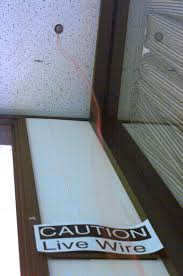
\includegraphics[width=0.3\linewidth]{introduction/live_wire.jpg}
    \caption{A Live Wire hanging from the ceiling (1996) \cite{weiser1996designing}.}
    \label{fig:live_wire}
\end{figure}

In the years following the conception of ubicomp, research and industry progressed far beyond the point of dangling strings. At the turn of the milennium we saw the emersion of digital clocks that not just display time but also the weather forecast, the room temperature, and other information. Of course, clocks were already a form of ubicomp in and of themselves, continuously telling the time without forcing the user's attention, and weather forecasts were available in a variety of ways. However, having all this information neatly summarized, available at a glance when we get up in the morning, was a clear step forward.

The next two decades gradually brought us smart lights, smart thermostats, smartphones, smartwatches, smart toothbrushes and smart toasters. All these devices have some sensors or a network connection with which they try to understand the context in which they are used, so as to better serve and anticipate the user's needs. In recent year, many companies, including Microsoft, Google, Apple, Amazon and Samsung, have all released their own digital assistant. These sophisticated programs can understand spoken natural language to some degree, and they can perform all kinds of tasks, from ordering takeaway to scheduling appointments. We find these assistants on our computers, our smartphones and on smart speakers we can place throughout our houses. No matter where we are, we can now complete many kinds of tasks simply by describing them. Combine this with the fact that we can now buy smart bathroom scales that will communicate with our smartwatches to find out how many calories we burned on a given day and automatically compare this to our change in weight, and we can see that computing is becoming truly ubiquitous.

The recent surge in complex ubicomp devices is no coincidence. For decades, a big obstacle, if not \textit{the} biggest one, in the further development of ubicomp, has been hardware capabilities \cite{abowd2000charting}. Low power consumption, solid wireless communication and excellent (touch) displays are but some of the requirements for enabling the seamless human-computer interaction that Weiser and others envisioned \cite{weiser1993some}. In recent years, these hurdles are being rapidly overcome. The widespread adoption of smartphones, which boast all three of the aforementioned requirements, is perhaps the most striking evidence thereof.

Development of a technology and research into its possible applications often go hand in hand, since the latter has little use without the former, and the former will create demand for the latter. With hardware limitations diminishing, other ubicomp challenges are becoming more prominent. Some current open research questions concern \textbf{intelligibility}, or how to make computer systems easy to understand, and visibility, or how to make users aware of the presence of these systems \cite{vermeulen2009bet,vermeulen2013intelligibility}. The fact that computer size is now becoming a concern for visibility, goes to show just how much progress has been made.

The solution to the usability problems of ubicomp might, somewhat counterintuitively, be to hide the computer entirely. The idea behind virtual reality (VR) and augmented reality (\textbf{AR}) is for the computer to become completely invisible by influencing the user's sensory input, which at the same time would allow it to communicate using any combination of the senses, like vision, hearing and touch \cite{rheingold1991virtual}. As such, the computer would be able to convey information intuitively and with any degree of intrusiveness, making the approach excellent for implementing the ubicomp ideals \cite{weiser1993some}.

So far, AR has remained a rather exclusive technology, with most applications either still in development, or requiring expensive or unwieldy hardware. The release of the mobile game Pokémon Go in 2016 is cited by many as the first time AR was brought to the general population \cite{HowPokem83:online}. The game is free and requires only a common smartphone, allowing nearly anyone to play. In the game, Pokémon are placed throughout the real world, and players can battle them while looking through their phone screen. The instant worldwide success of this game encouraged the development of many more AR applications and made people familiar with the technology. Around the same time, Snapchat introduced their popular Lens feature, which used facial recognition to change people's faces in real-time, usually to add funny animations. In 2017, they added the ability for 3D objects, like animated characters, to be anchored into space within these video's \cite{Snapchat36:online}.

With ubicomp and AR both quickly becoming practical, affordable and widespread, we believe this is a very opportune time to investigate how they can work together in meaningful ways. Much research remains to be done for each technology in and of itself, let alone for their combination \cite{liberati2016augmented}. Most existing ubicomp AR devices, like the Google Glass, the Microsoft HoloLens and the Magic Leap One, are as of yet still advertised, and priced, towards developers and enterprises \cite{Wearable31:online,Microsof18:online,MagicLea40:online}. While not yet in the hands of the end-users, they are available to us for rapid prototyping and easy experimentation. Considering how young and quickly evolving these technologies still are \cite{liberati2016augmented}, we are given a great opportunity indeed.

An important challenge of ubicomp concerns the fact that, while actions in virtual environments are often reversible, the real world is much less forgiving. File edits can be undone, videos can be rewound and computers can be reset, but smart ovens cannot unburn a meal, smart garage doors cannot unscratch a car and smart lights cannot unwake a baby. For this reason, it is essential to inform users in ubicomp scenarios on what actions will achieve which effect. This process of telling the user what is going to happen if they proceed with an action is called \textbf{feedforward}. It is the future-equivalent of feedback, which is the process showing the user the result of an action after they executed it.

Feedforward is a powerful tool, as it has repeatedly been shown to improve user's confidence in their actions and trust in the system \cite{vermeulen2009bet, park2014previewable}, and to improve user's understanding of the system \cite{bau2008octopocus, vermeulen2009bet, vermeulen2012understanding, vermeulen2013intelligibility}. However, research is still young \cite{vermeulen2013crossing}, and the technique remains relatively unused. This is illustrated by the fact that, while \textit{feedback} is a commonly used word, the term \textit{feedforward} is rarely found outside of research. In conventional computers, the existence of undo buttons might have limited the need for feedforward to become a standard interface design tool, but the move to ubicomp does not allow for trial-and-error-based interactions to remain common practice.

As mentioned before, visibility of systems is a problem that was less prominent before the rise of ubicomp. In conventional computing, all relevant components are usually right in the user's hands or on a screen right in front of them, but in ubicomp environments, interactive devices can by definition be located anywhere. Still, giving each component a clearly visible location in space is important. Users grow more confident, show more trust and find systems easier to understand when each device has a clearly designated spot, even if the location is arbitrary, like with a voice-controlled assistant \cite{vermeulen2009bet}. Furthermore, devices are often interconnected, like lights connected to a motion sensor, or a door knob connected to the central security panel. Since each component has a location in space, and since multiple components can be related, spatial awareness is an important asset in conveying the functionality of an environment to the user. Without an understanding of which object is located where in space, the system must resort to labels, descriptions, pictures and the likes to point out devices. In contrast, with spatial understanding, and a means of augmenting the the environment, we suspect better options become available.

The aim of this thesis is to find and evaluate new visualizations for spatial awareness in ubicomp environments. Devices like the HoloLens enable us to track the user's movement, understand what they are looking at, and augment their vision in real time. We want to use this technology to create visualizations for spatial awareness which, given some event or action, provide feedforward by helping to find all the relevant components. For example, given a row of light switches, we can provide feedforward by showing where the lights are located that will turn on when each of the switches is pressed. When the user is about to accidentally trigger their home alarm, we can point out the sensor and mark the area to avoid. When the user stands in front of their fuse box, we can visualize which areas of the house are connected to which fuse. Our hypothesis is that these visualizations will improve user confidence, trust and understanding of the system.

We begin this thesis with a literature study of related work in Chapter \ref{chap:relat}. We discuss existing interaction techniques related to ubicomp, AR, feedforward, or some combination of the three, and we analyze the results of past experiments on these topics. Building upon this knowledge, we follow up with our own exploration of the design space in Chapter \ref{chap:explor}. We perform this exploration by designing our own set of visualizations, which we evaluate via an online survey. Armed with the conclusions of this survey, we create a working prototype of the most promising visualizations, using the Microsoft HoloLens, the implementation of which is described in Chapter \ref{chap:impl}. Chapter \ref{chap:user} discusses the user study we performed with this prototype. Finally, in Chapter \ref{chap:concl} we formulate our conclusions for this thesis and note possible future work.

%\todo{Talk about the history of AR.}

%Another challenge in ubicomp concerns the fact that, while actions in virtual environments are often reversible, the real world is much less forgiving. For this reason, it's essential to inform users of what actions will achieve which effect in a process called \textbf{feedforward} \cite{djajadiningrat2002but}. While the notion of feedforward is both powerful and important, much research on the topic remains to be done \cite{vermeulen2013crossing}.

%In this thesis, we investigate the potential of AR for giving feedforward on ubicomp systems, with the goal of improving their intelligibility. More specifically, we look for intuitive cues that can inform the user on the result of each possible action they can take in a given environment. Feedforward via senses other than vision, such as auditory or tactile input, are not considered.

%\todo{The description of chapters below must be adjusted.}

%Chapter \ref{chap:explor} commences this thesis with a study of related work. We look at interaction techniques concerning AR, feedforward and ubicomp that are suggested by other research teams and analyze the results of past experiments on these topics. Using that information, we look for an interesting problem on which we can perform an in-depth study for the remainder of this thesis.

%The problem that we decide on is the spatial mapping problem of light switches, or the question of which lights are connected to which switches in a given room (and vice versa). We chose this problem because it is both relevant and recognizable, since many people need to solve such problems on a regular basis, and because it allows us to easily come up with scenarios of arbitrary complexity.

%Our next step is to gather initial data on a wide variety of solutions so as to better focus the remainder of our study. To this end, we distribute an online survey containing seven different visualizations, and for each of them, we measure the performance and perception of the respondents. The setup, execution, results and conclusions of this preliminary study are discussed in chapter \ref{chap:explor}.

%In 1988, when I started PARC’s work on ubiquitous computing, virtual reality (VR) came the closest to
%enacting the principles we believed important. In its ultimate envisionment, VR causes the computer to
%become effectively invisible by taking over the human sensory and affector systems [Rheingold 91]. VR
%is extremely useful in scientific visualization and entertainment, and will be very significant for those
%niches. But as a tool for productively changing everyone’s relationship to computation, it has two crucial
%flaws: first, at the present time (1992), and probably for decades, it cannot produce a simulation of
%significant verisimilitude at reasonable cost (today, at any cost). This means that users will not be fooled
%and the computer will not be out of the way. Second, and most importantly, it has the goal of fooling the
%user -- of leaving the everyday physical world behind. This is at odds with the goal of better integrating
%the computer into human activities, since humans are of and in the everyday world. \cite{weiser1993some}

%Human-computer interaction has come a long way since the first computers were created around 75 years ago. 
%We've come a long way since the invention of computers
%Interfaces have changed a lot, and now, like the devices they belong to, they're becoming ubiquitous.
%New interface require new techniques
%Many techniques have been developed over the years: affordances and signifiers, (continuous) feedback and feedforward
%Actions in the real world are not always as reversible as they are in the virtual world.

%\section{Feedforward} \label{section_background}
%Feedforward is a relatively new concept that has been the subject of much confusion, and thus it is worth clarifying. Feedforward was first defined by \citeauthor{djajadiningrat2002but} in \citeyear{djajadiningrat2002but} as 
%
%
%Feedforward is:
%	communication of the purpose of an action. \cite{djajadiningrat2002but}
%
%	informs the user about what the result of his action will be. Inviting the appropriate action is a prerequisite for feedforward but it is not sufficient. The product also needs to communicate what the user can expect. \cite{djajadiningrat2002but}
%
%	a HCI design technique that aims at making explicit the action that is required to perform an interaction and its effect. \cite{chueke2016perceptible}
%	
%	intelligibility information that is provided before an event takes place. \cite{vermeulen2013intelligibility}
%	
%	communicating what will be the result of an action


%Feedforward hasn't always been clearly defined. People don't know it exists, confuse it with other concepts (like affordances) or use different names for it (signifiers). Let's now define what feedforward is, according to different definitions.
%
%Perceptible affordances and feedforward for gestural interfaces: Assessing effectiveness of gesture acquisition with unfamiliar interactions \cite{chueke2016perceptible}
%
%Intelligibility Required: How to Make Us Look Smart Again \cite{vermeulen2013intelligibility}
%
%Crossing the bridge over Norman's Gulf of Execution: revealing feedforward's true identity \cite{vermeulen2013crossing}
%
%When it is not possible for designers of electronic products to establish direct couplings between action and function information is needed. Information that can guide the user’s actions towards the intended function. This is the area of feedback and feedforward. \cite{wensveen2004interaction}
%
%With feedforward we mean communication of the purpose of an action. \cite{djajadiningrat2002but}
%
%For a control to say something about the function that it triggers, we need to move away from designs in which all controls look the same. \cite{djajadiningrat2004tangible} 
%
%As pointed out by Norman \cite{norman2013design}, controls of electronic products often look highly similar and require the same actions. If all controls look the same and feel the same, the only way left to make a product communicate its functions is through icons and text labels, requiring reading and interpretation. \cite{djajadiningrat2004tangible}
%
%Signifiers are the most important addition to the chapter, a concept first introduced in my book Living with Complexity. The first edition had a focus upon affordances, but although affordances make sense for interaction with physical objects, they are confusing when dealing with virtual ones. As a result, affordances have created much confusion in the world of design. Affordances define what actions are possible. Signifiers specify how people discover those possibilities: signifiers are signs, perceptible signals of what can be done. Signifiers are of far more importance to designers than are affordances. Hence, the extended treatment. \cite{norman2013design}
%
%Preview important in the real world because it is often not possible to undo an action. \cite{rekimoto2003presense}
